\section{Overview}

\subsection{Agency}

\begin{enumerate}
    \item Ask: is the principal liable to a third party for another's actions?
    \item \textbf{Three actors}: principal, agent, third party. The third 
    party is bringing the claim.
    \item Two types of cases: \textbf{contract} and \textbf{tort}.
    \item Is there an \textbf{agency relationship}? Elements:\footnote{See 
    Restatement (Third) \S\ 1.01. This step of the analysis applies to both 
    contract and tort cases.}
    \begin{enumerate}
        \item The principal's \textbf{manifestation of assent}. (This can 
        exist even if the principal explicitly denies an agency relationship. 
        The terminology of the agreement is not controlling.\footnote{Casebook 
        p. See, e.g., \emph{Cargill}, where the lawyers disclaimed an agency 
        relationship in the initial agreement.})
        \item Agent acting on the principal's \textbf{behalf}. (Do the agent's 
        actions directly benefit the principal?)
        \item Agent subject to the principal's \textbf{control}.
        \item Agent \textbf{consents}.
        \item Examples:
        \begin{enumerate}
            \item Setting the \textbf{purpose and conditions} of activity can 
            establish an agency relationship. \emph{Gorton v. Doty}, p.  
            \pageref{subsub:gorton}.
            \item A creditor that exercises enough control over a debtor's 
            business can be liable as a principal for the debtor's acts. 
            \emph{A. Gay Jenson Farms Co. v. Cargill}, p. 
            \pageref{subsub:cargill}.
        \end{enumerate}
    \end{enumerate}
    \item If this is a \textbf{breach of contract} case:
    \begin{enumerate}
        \item Did the agent have \textbf{authority} to act? Types of authority 
        (which often overlap):\footnote{This step applies \emph{only} to 
        contract cases.}
        \begin{enumerate}
            \item \textbf{Actual}: can be (1) express or (2) implied. \S\S\ 
            2.01--2.02.
            \item \textbf{Apparent}: did the third party reasonably believe 
            the agent had authority, and was that belief \emph{traceable} to 
            the principal's manifestations? \S\ 2.03.
            \item (These often overlap---e.g., \emph{Mill Street Church}, p.  
            \pageref{par:mill}.)
        \end{enumerate}
        \item Do any \textbf{exceptions} apply?\footnote{These are substitutes 
        for authority.}
        \begin{enumerate}
            \item \textbf{Ratification}: requires the principal's (1) 
            \textbf{intent to ratify} and (2) \textbf{full knowledge} of 
            material circumstances. \emph{Botticello v. Stefanovicz}, p.  
            \pageref{par:botticello}. See also Restatement (Third) \S\S\ 4.01 
            (definition), 4.02 (effect), and 4.05(1) (timing).
            \item \textbf{Estoppel}: a third party can assert estoppel when 
            he (1) \textbf{detrimentally relies} on an impostor agent and (2) 
            the principal \textbf{intentionally or carelessly} caused the 
            belief or the principal \textbf{was on notice} and failed to take 
            reasonable steps. Restatement (Third) \S\ 2.05 and 
            \emph{Hoddeson}, p. \pageref{par:hodd}.
            Estoppel only creates liability for the 
            principal (i.e., the principal can't assert estoppel against the 
            third party).
            \item \textbf{Undisclosed principal}: if the agent lacks 
            authority (either actual or apparent), the undisclosed principal 
            can still be liable for acts that are ``within the authority 
            usually confided'' to agents. See \emph{Watteau}, p. 
            \pageref{par:watteau}. Requires an underlying agency 
            relationship.
        \end{enumerate}
    \end{enumerate}
    \item If this is a \textbf{tort} case:
    \begin{enumerate}
        \item \textbf{Respondeat superior}: employers are liable for torts 
        their \textbf{employees} commit while within the \textbf{scope of 
        employement}. Restatement (Third) \S\ 2.04.
        \begin{enumerate}
            \item \textbf{Definition of employee}: is an agent (under 
            Restatement \S\ 1), and the principal controls or has the right to 
            control the \textbf{manner and means} of the work. Restatement 
            (Third) \S\ 7.07(3).
            \begin{enumerate}
                \item Servant/employee: principal is liable for torts if the 
                employee was acting within the scope of employment.
                \item Independent contractor (agent-type): P is liable for 
                contracts but not torts.
                \item Independent contractor (non-agent): P is not liable.
            \end{enumerate}
            \item \textbf{Definition of scope of employement}: doesn't include 
            independent courses of conduct not intended to serve the 
            employer's purposes. Restatement (Third) \S\ 7.07.  
            \end{enumerate}
        \item \textbf{Exceptions} (under which P is liable):
        \begin{enumerate}
            \item Engaging an incompetent contractor.
            \item Nondelegable duty.
        \end{enumerate}
        \item \textbf{Employees vs. independent contractors} (Restatement 
        (Second) \S\ 220(2)):
        \begin{enumerate}
            \item P \emph{may} exercise control over details of A’s work
            \item A does not engage in distinct business
            \item Type of work typical of supervised employee, not unsupervised specialist
            \item Job requires low skill level
            \item P supplies tools and dictates place of work
            \item A employed for a long term
            \item A is compensated by time and not by job
            \item Work is a regular part of P’s business
            \item Intent to create employer/employee relationship
            \item P is in business
            \item See gas station cases (\emph{Humble} and \emph{Sun Oil}) for 
            similar facts reaching different conclusions on the 
            employee-vs.-independent-contractor question.
        \end{enumerate}
        \item \textbf{Franchises}: a standard franchise system does not 
        necessarily establish an employee relationship (\emph{Murphy}), but it 
        can if the franchisees are tightly controlled (\emph{McDonald's).}
        \item \textbf{Apparent authority}: arises when the principal 
        represents that another is his servant or other agent and causes the 
        third person to rely upon the \textbf{care or skill} of the apparent 
        agent. Does not require an agency relationship under \S\ 1. 
        \emph{McDonald's}.
        \begin{enumerate}
            \item Why is this different than apparent \emph{agency}? Because 
            authority doesn't apply to tort cases. Torts are about 
            \emph{mistakes}, not \emph{instructions}. Principals rarely 
            authorize their agents to commit torts.
        \end{enumerate}
    \end{enumerate}
    \item \textbf{Agent liability}:
    \begin{enumerate}
        \item A is liable for his own torts.
        \item A is liable in contract when:
        \begin{enumerate}
            \item Acting without authority (because of the implied warranty).
            \item When acting for an undisclosed or unidentified principal.
        \end{enumerate}
        \item A is liable to the principal for breach of fiduciary duty.
    \end{enumerate}
    \item \textbf{Agent's fiduciary duties}:
    \begin{enumerate}
        \item Loyalty.
        \begin{enumerate}
            \item Material benefit arising out of position.
            \item Acting as or on behalf of adverse party.
            \item Competition.
            \item Use of principal's property \& confidential info.
        \end{enumerate}
        \item Care, competence, and diligence.
        \item Act within scope of authority.
    \end{enumerate}
    \item \textbf{Strategies for avoiding liability}:
    \begin{enumerate}
        \item (First, define the \textbf{risks and rewards}.)
        \item Get \textbf{insurance}. \emph{Gorton v. Doty}, p.
        \pageref{subsub:gorton}.
        \item \textbf{Legal structuring}: structure the relationship to negate 
        one of the four elements.
        \begin{enumerate}
            \item Specify the nature of the relationship, ideally in writing.
            \item Delegate control to another principal, or give up control 
            entirely.
        \end{enumerate}
        \item \textbf{Security/collateral}. E.g., a right of first refusal. 
        \emph{A. Gay Jenson Farms Co. v. Cargill}, p.  
        \pageref{subsub:cargill}. \emph{Cargill}.
        \item \textbf{Monitoring}. E.g., accounting audits.
        \item \textbf{Operational control}. E.g., a sign-off requirement for 
        major decisions. \emph{Cargill} again.
        \item \textbf{Due diligence}. E.g., verify the type of property 
        interest that the seller is selling. \emph{Botticello v. Stefanovicz}, 
        p. \pageref{par:botticello}.
        \item \textbf{Recording/registration systems}. E.g., check public land 
        records. \emph{Botticello}.
    \end{enumerate}
    % Include Cable chart
    \includepdf{resources/agency.pdf}
\end{enumerate}

\newpage

\subsection{Partnership}

\begin{enumerate}
    \item \textbf{What is a partnership and who are the partners?}
    \begin{enumerate}
        \item ``The association of two or more persons to carry on as 
        co-owners a business for profit forms a partnership, whether or not 
        the persons intended to form a partnership.'' RUPA \S\ 202(a)
        \item \textbf{Profit sharing} and \textbf{management rights} weigh in 
        favor of the existence of a partnership. But profit sharing alone 
        without sharing in losses is not enough to establish a partnership. 
        \emph{Fenwick}, p. \pageref{par:fenwick-ucc}.
        \item The partners' \textbf{intent} is not determinative.
        \item All partners are \textbf{jointly and severally liable} for all 
        obligations of the partnership. RUPA \S\ 305.
        \item Partnership by \textbf{estoppel}:
        \begin{enumerate}
            \item \textbf{Representation/holding out} that one person is the 
            partner of another.
            \item Representation came from the \textbf{defendant}.
            \item Plaintiff \textbf{relied}, reasonably and in good faith, on 
            the representation.
            \item The plaintiff suffered a \textbf{detrimental change in 
            position} based on that reliance.
            \item See \emph{Young v. Jones}, p. \pageref{par:young}, finding 
            no partnership by estoppel.
        \end{enumerate}
    \end{enumerate}
    \item \textbf{Partners' fiduciary duties}:
    \begin{enumerate}
        \item Partners owe a duty to other partners. \emph{Meinhard v. 
        Salmon}, p. \pageref{par:meinhard}.
        \item RUPA \S\ 404 seems to require a duty to \textbf{share} in 
        partnership opportunities.
    \end{enumerate}
    \item \textbf{Rights of partners}:
    \begin{enumerate}
        \item Each partner is an agent of the partnership with equal rights. 
        RUPA \S\S\ 301(1), 401(f). \emph{National Biscuit v. Stroud}, \pageref{par:biscuit}.
        \item Limiting one partner's authority requires a majority vote. RUPA 
        \S\ 401(j). But one partner is not a majority. Two-person partnerships 
        can end in deadlock. \emph{Summers v. Dooley}, p. 
        \pageref{par:summers}.
    \end{enumerate}
\end{enumerate}

\newpage

\subsection{Corporate Formation}

\begin{enumerate}
    \item \textbf{Corporate structure}.
    \begin{enumerate}
        \item \textbf{Public}: many public shareholders, liquid shares, traded 
        on an exchange.
        \item \textbf{Private} or \textbf{closely held}: few shareholders, 
        shareholders are also officers and directors, shares are hard to sell.
        \item \textbf{Dividens}: paid at the board's discretion.
    \end{enumerate}
    \item \textbf{Formation}.
    \begin{enumerate}
        \item \textbf{Articles of incorporation}: incorporator (often a 
        lawyer) files and then (1) organizes the company herself or (2) names 
        initial directors, who then do the rest. MBCA \S\ 2.05.
        \item \textbf{Capital structure}: authorized shares---common stock, 
        preferred stock. MBCA \S\S\ 6.01--02.
        \item \textbf{Organizational consent} (at a meeting or by written 
        consent): adopt bylaws, elect officers, conduct ``other business.'' 
        MBCA \S\ 2.05.
        \item \textbf{Bylaws}: repeat provisions from statute and articles; 
        governance procedures; officer duties and authority; rules for bylaw 
        amendments. MBCA \S\ 2.06.
        \item \textbf{Officer appointments}: few requirements, although some 
        states require president, secretary, etc. MBCA \S\ 8.40.
        \item \textbf{Stock issuance}: \textbf{subscription} (agreement to 
        purchase on specified terms) or \textbf{issuance} (ritual of 
        certificating and entering on stock register). MBCA \S\S\ 6.20--21.
        \item \textbf{Shareholders' agreement}: a private contract among 
        shareholders.
        \item \textbf{Annual election of officers and directors}, as required 
        by statute.
    \end{enumerate}
    \item \textbf{Limited liability}.
    \begin{enumerate}
        \item \textbf{Enterprise liability}:
        \begin{enumerate}
            \item Holds sister corporations liable when money, operations, and 
            employees are commingled.
            \item Good record-keeping can avoid commingling.
        \end{enumerate}
        \textbf{Piercing the corporate veil} can result from:
        \begin{enumerate}
            \item \textbf{Unity of interest and ownership} between a 
            shareholder and corporation (i.e., sloppiness):
            \begin{enumerate}
                \item Not following \textbf{formalities}; or
                \item \textbf{Commingling} corporate and personal business; or
                \item \textbf{Undercapitalization};
            \end{enumerate}
            \item Or \textbf{promotion of injustice}:
            \begin{enumerate}
                \item \textbf{Fraudulent conduc} (e.g., promising payment 
                while draining assets); or
                \item \textbf{Unjust enrichment}.
            \end{enumerate}
            \item % TODO add walkovsky -- taxi case
        \end{enumerate}
        \item \textbf{Dividend rules}:
        \begin{enumerate}
            \item Corporations must be able to \textbf{pay creditors} before 
            issuing dividends. MBCA \S\ 6.40.
            \item Directors are \textbf{personally liable} for impermissible 
            dividends. MBCA \S\ 8.33.
        \end{enumerate}
        \item \textbf{Reverse piercing}:
        \begin{enumerate}
            \item Assume no enterprise liability.
            \item Apply PVC test downward to to reach the assets of a 
            subsidiary. \emph{Sea-Land}. % TODO add xref
            % Include `deep pockets' exam review chart
            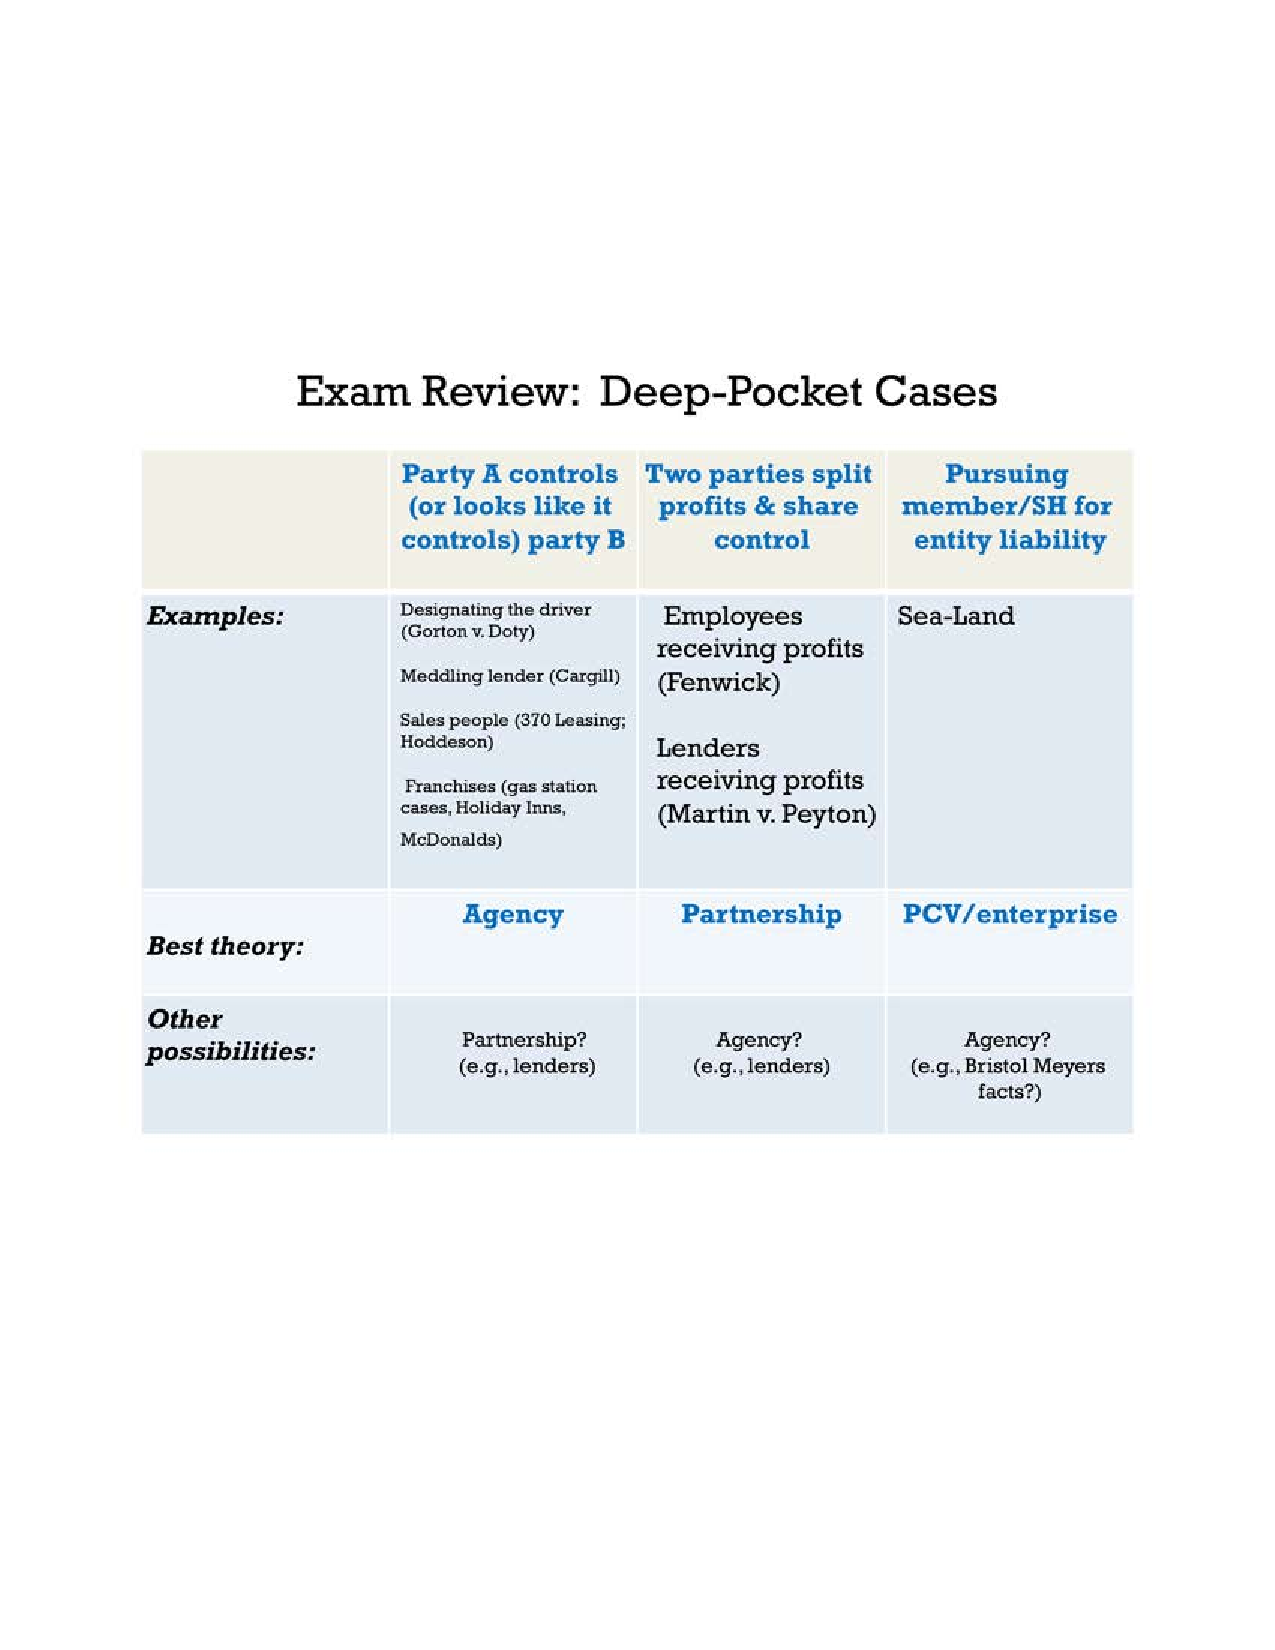
\includepdf{resources/deep-pockets.pdf}
        \end{enumerate}
    \end{enumerate}
    \item \textbf{Role and purpose of the corporation}.
    \begin{enumerate}
        \item Courts are deferential to corporate philanthropy, as long as the 
        corporation avoids \textbf{pet charities}, the donations are 
        \textbf{modest}, and the corporation has a reasonable belief that the 
        donation will \textbf{advance the corporation's interest}. \emph{AP 
        Smith}. % TODO add xref
        \item The donation must have \textbf{some corporate purpose}. You 
        can't just give away money. \emph{Dodge}. % TODO add xref
        \item \textbf{Business judgment rule}: ``Courts will not step 
        in and interfere with honest business judgment of the directors unless 
        there is a showing of fraud, illegality, or conflict of interest.'' 
        \emph{Shlensky v. Wrigley}. % TODO add xref
    \end{enumerate}
\end{enumerate}

\newpage

\subsection{Limited Liability Company}

\begin{enumerate}
    \item \textbf{Limited partnership}:
    \begin{enumerate}
        \item \textbf{Limited} (passive) partners: not personally liable for 
        partnership liabilities.
        \item \textbf{General} (active) partners:
        \begin{enumerate}
            \item Personally liable.
            \item \textbf{At least one required}.
            \item Can be an entity---e.g., VC funds are sometimes organized as 
            LPs with an LLC as the general partner.
        \item Whether someone is a limited or general partner depends on the 
        level of active involvement---e.g., selecting crops to plant, 
        overruling the general partner, signing checks, firing a manger. 
        \emph{Holzman v. De Escamilla}. % TODO add xref
        \end{enumerate}
    \end{enumerate}
    \item \textbf{Limited liability partnership}:
    \begin{enumerate}
        \item Formation: file with the state.
        \item Management rights: partners have the rights of general partners 
        (not passive partners).
        \item Liability: some states limit liability for torts only (not 
        contracts).
        \item Eligibility: professional services (engineers, lawyers, etc.).
    \end{enumerate}
    \item \textbf{Limited liability company}:
    \begin{enumerate}
        \item \textbf{Overview}:
        \begin{enumerate}
            \item \textbf{Nutshell}: Tax advantages of a partnership; limited 
            liability of a corporation; management structure somewhere in 
            between.
            \item \textbf{History}: introduced in late 70s, tax status settled 
            in late 90s.
            \item \textbf{Tax}:
            \begin{enumerate}
                \item \textbf{No double taxation} on operating profits and 
                losses; they \textbf{flow through} to owners.
                \item Easy for an LLC to convert to a corporation, but not the 
                other direction because of the \textbf{tax trap}.
            \end{enumerate}
            \item \textbf{S-corporation}:
            \begin{enumerate}
                \item Regular corporation under state statutes, but with 
                special IRS paperwork.
                \item \textbf{Flow-through} taxation.
                \item 100 shareholder limit.
                \item Entities can't own shares.
                \item No preferred stock.
                \item For the last three reasons, \textbf{VCs disfavor 
                s-corps.}
            \end{enumerate}
            \item \textbf{Formation}:
            \begin{enumerate}
                \item File \textbf{articles of organization}.
                \item Establish \textbf{operating agreement}.
            \end{enumerate}
            \item \textbf{Membership}:  
            \begin{enumerate}
                \item \textbf{Owners} are ``members.''
                \item Default financial structure is similar to that of a 
                partnership.
            \end{enumerate}
            \item \textbf{Management}:
            \begin{enumerate}
                \item \textbf{Member-managed} (default rules):
                \begin{itemize}
                    \item Equal management rights.
                    \item Majority vote decides most matters.
                    \item Unanimity required for extraordinary matters (e.g., 
                    merger, dissolution).
                    \item Operating agreements often modify the default rules.
                \end{itemize}
                \item \textbf{Manager-managed}:
                \begin{itemize}
                    \item Multiple managers allowed.
                    \item Equal management rights.
                    \item Majority manager vote decides most issues.
                    \item Majority \emph{member} vote required for 
                    extraordinary matters.
                    \item Managers don't have to be members.
                \end{itemize}
            \end{enumerate}
            \item \textbf{Transferability}:
            \begin{enumerate}
                \item Similar rules to those in partnership.
                \item Members can assign their \textbf{economic} interest. 
                \item Admission of new members requires consent of all other 
                members.
                \item Operating agreements usually have buyout and buy-sell 
                provisions.
            \end{enumerate}
            \item \textbf{Fiduciary duties}: see below.
            \item \textbf{Limited liability}:
            \begin{enumerate}
                \item Limited under ULLCA \S\ 303(a).
                \item Veil can be pierced---see below.
            \end{enumerate}
        \end{enumerate}
        \item \textbf{Operating agreements}:
        \begin{enumerate}
            \item Indicate whether \textbf{member-managed or manager-managed}.
            \item Change \textbf{management rights} (the default is equal 
            rights under ULLCA \S\ 404).
            \item Change which members are \textbf{agents} (default: all are; 
            ULLCA \S\ 301). Each member in a member-managed LLC has 
            \textbf{statutory apparent authority} to bind the LLC for 
            ``business of the kind'' that the LLC engages in. ULLCA \S\ 301.
        % TODO elf v jaffari
        % TODO fisk v segal
        \end{enumerate}
        \item \textbf{Piercing the LLC veil}---generally the same as PCV. See 
        ULLCA \S\ 303(b) on formalities. Veil can be pierced when:
        \begin{enumerate}
            \item \textbf{Unity of interest and ownership}:
            \begin{itemize}
                \item Lack of formalities.
                \item Commingling of funds or assets.
                \item Under-capitalization.
            \end{itemize}
            \item \textbf{Injustice}:
            \begin{itemize}
                \item Fraud-like conduct.
                \item Unjust enrichment.
            \end{itemize}
        % TODO kaycee
        \end{enumerate}
        \item \textbf{Fiduciary duties}:
        \begin{enumerate}
            \item \textbf{Member-managed}:
            \begin{enumerate}
                \item All members have duties of loyalty and care.
            \end{enumerate}
            \item \textbf{Manager-managed}:
            \begin{enumerate}
                \item Managers have duties of care and loyalty.
                \item Members have no duties in their role as members.
            \end{enumerate}
        % TODO mcconnell
        \end{enumerate}
    \end{enumerate}
\end{enumerate}

\newpage

\subsection{Board of Directors}

\begin{enumerate}
    \item \textbf{Business judgment rule}:
    \begin{enumerate}
        \item Court will not substitute its judgment for the board's unless 
        the plaintiff can show that:
        \begin{enumerate}
             \item The board was \textbf{grossly negligent in becoming 
             informed}---a breach of the \emph{duty of care}.
             \item The board acted with \textbf{bad faith} or engaged in 
             \textbf{self-dealing}---a breach of the \emph{duty of loyalty}.
        \end{enumerate}
        \item If the plaintiff can rebut the business judgment rule, the court 
        will review the transaction under \textbf{entire fairness}.
        \item Intermediate scrutiny applies in special contexts---(1) takeover 
        defenses (\emph{Unocal}) and sales of control (\emph{Revlon}).
    \end{enumerate}
    \item \textbf{Duty of care}:
    \begin{enumerate}
        \item \textbf{Definition}: directors must act with the diligence of a 
        reasonable person under similar circumstances.
        \item Plaintiffs are not liable for a breach of the duty of care 
        unless the plaintiff can prove ``fraud, dishonesty, or nonfeasance.'' 
        \emph{Kamin v. American Express}. % TODO xref
        \item \textbf{Types of deals}:
        \begin{enumerate}
            \item \textbf{Stock purchase}: acquirer buys enough stock from 
            shareholders to gain control of a target company.
            \item \textbf{Cash merger}: like a stock purchase, but the 
            acquirer then merges with the target. 
            \item \textbf{Triangular merger}: acquirer buys target and then 
            merges it with a subsidiary of the acquirer.
            \item \textbf{Basic asset sale}: acquirer buys assets directly 
            from the target.
            \item \textbf{Leveraged buyout}: a company is acquired using 
            borrowed money.
        \end{enumerate}
        \item Plaintiffs can rebut the BJR presumption by showing that the 
        board was \textbf{grossly negligent in becoming informed} before 
        making a business decision. \emph{Smith v. Van Gorkom}. % TODO xref
        \item Articles (or certificate) of incorporation can \textbf{eliminate 
        personal liability} for duty of care breaches (but not for breaches of 
        duty of loyalty or good faith). DGCL \S\ 102(b)(7).
    \end{enumerate}
    \item \textbf{Duty of loyalty}:
    \begin{enumerate}
        \item \textbf{Directors' and managers' conflicts}:
        \begin{enumerate}
            \item \textbf{Three ways to cleanse a self-dealing transaction} 
            under DGCL \S\ 144(a):
            \begin{enumerate}
                \item Approval by a \textbf{majority of disinterested 
                directors}. \emph{Benihana}. % TODO add xref
                \item Approval by \textbf{shareholders}.\footnote{Must the 
                shareholders be disinterested? DGCL 144(a) requires \emph{all} 
                shareholders, but the \emph{Fliegler} court (in DE) required 
                only \emph{disinterested} shareholders. MBCA \S\ 8.60 ff. also 
                requires disinterested shareholders.}
                \item \textbf{Entire fairness}. \emph{Bayer v. Beran}, below.
                \item (Approving directors or shareholders must be 
                \textbf{fully informed}.)
            \end{enumerate}
            \item Courts will review self-dealing transactions under entire 
            fairness using the following factors (\emph{Bayer v. Beran}): % TODO xref
            \begin{enumerate}
                \item Cost of the transaction vs. the industry standard.
                \item Cost vs. company revenues.
                \item Compensation of the interested client (here, the 
                director's wife) vs. other similar non-interested clients.
                \item Use of form contracts.
                \item Whether the transaction was negotiated through an agent.
                \item The apparent success of the transaction.
            \end{enumerate}
        \end{enumerate}
        \item \textbf{Corporate opportunities}:
        \begin{enumerate}
            \item \textbf{Tender offer}: acquirer offers to buy as many shares 
            of a target as it can. Goal is control of the target.
            \item \textbf{Corporate opportunity test} (if yes, the director 
            must offer the opportunity to the corporation) (\emph{Broz}): % TODO xref
            \begin{enumerate}
                \item Does the corporation have the \textbf{financial 
                capability} to pursue the opportunity?
                \item Is the opportunity in the corporation's \textbf{line of 
                business}?
                \item Does the corporation have an \textbf{interest or 
                expectancy} in the opportunity?
                \item Would the director's pursuit of the opportunity 
                \textbf{lead to conflicts} (e.g., competition or use of 
                confidential inside information)?
            \end{enumerate}
            \item No duties owed to a potential acquiror.
            \item \textbf{Competition}: directors and officers can't compete 
            with the corporation except (1) when the benefits outweigh the 
            harm or (2) when approved.
        \end{enumerate}
        \item \textbf{Dominant shareholders}:
        \begin{enumerate}
            \item Intrinsic fairness (essentially, entire fairness) applies 
            when a dominant shareholder \textbf{engages in 
            self-dealing}---i.e., when the dominant shareholder receives 
            something ``to the exclusion of, and detriment to, the minority 
            stockholders'' of the corporation (often, a subsidiary). 
            \emph{Sinclair Oil v. Levien}.
        \end{enumerate}
        \item \textbf{Ratification/voting}:
        \begin{enumerate}
            \item See drafting exercises.
            \item \textbf{Two voting standards} at a meeting under DGCL:
            \begin{itemize}
                \item \textbf{General transactions} (e.g., approving 
                auditors) (DGCL \S\ 216):
                \begin{enumerate}
                    \item \emph{Quorum}: majority of shares entitled to vote 
                    in person or by proxy.
                    \item \emph{Approval}: majority of shares \textbf{present 
                    in person or by proxy at the meeting}.
                \end{enumerate}
                \item \textbf{Merger} (\S\ 251):
                \begin{enumerate}
                    \item Same.
                    \item Majority of \textbf{all outstanding shares}.
                \end{enumerate}
            \end{itemize}
            \item \textbf{Notice of board meeting}: MBCA \S\ 8.22 provides 
            default rules, but \textbf{articles or bylaws can override them}.
            \item \textbf{Shareholders' written consent}: MBCA \S\ 7.04(a) 
            \textbf{trumps bylaws}.
        \end{enumerate}
    \end{enumerate}
    \item \textbf{Good faith}:
    \begin{enumerate}
        \item Two types of cases: \textbf{overcompensation} (\emph{Disney}) 
        and \textbf{oversight} (\emph{Caremark}).
        \item Why does it matter?
        \begin{enumerate}
            \item Only directors acting in good faith are entitled to 
            indemnification. DGCL \S\ 145.
            \item Articles cannot eliminate liability for bad faith conduct. 
            DGCL 102(b)(7).
        \end{enumerate}
        \item Large executive compensation is not usually enough to establish 
        bad faith or waste. \emph{Disney}.
        \item Directors can be liable for \textbf{lack of oversight} if (1) 
        they fail to implement a reporting system or controls; or (2) if they 
        have implemented such systems or controls, ``consciously failed to 
        monitor or oversee its operations thus disabling themselves from being 
        informed of risks or problems requiring their 
        attention.''\footnote{Casebook p. 395.} \emph{Stone v. Ritter}.
    \end{enumerate}
    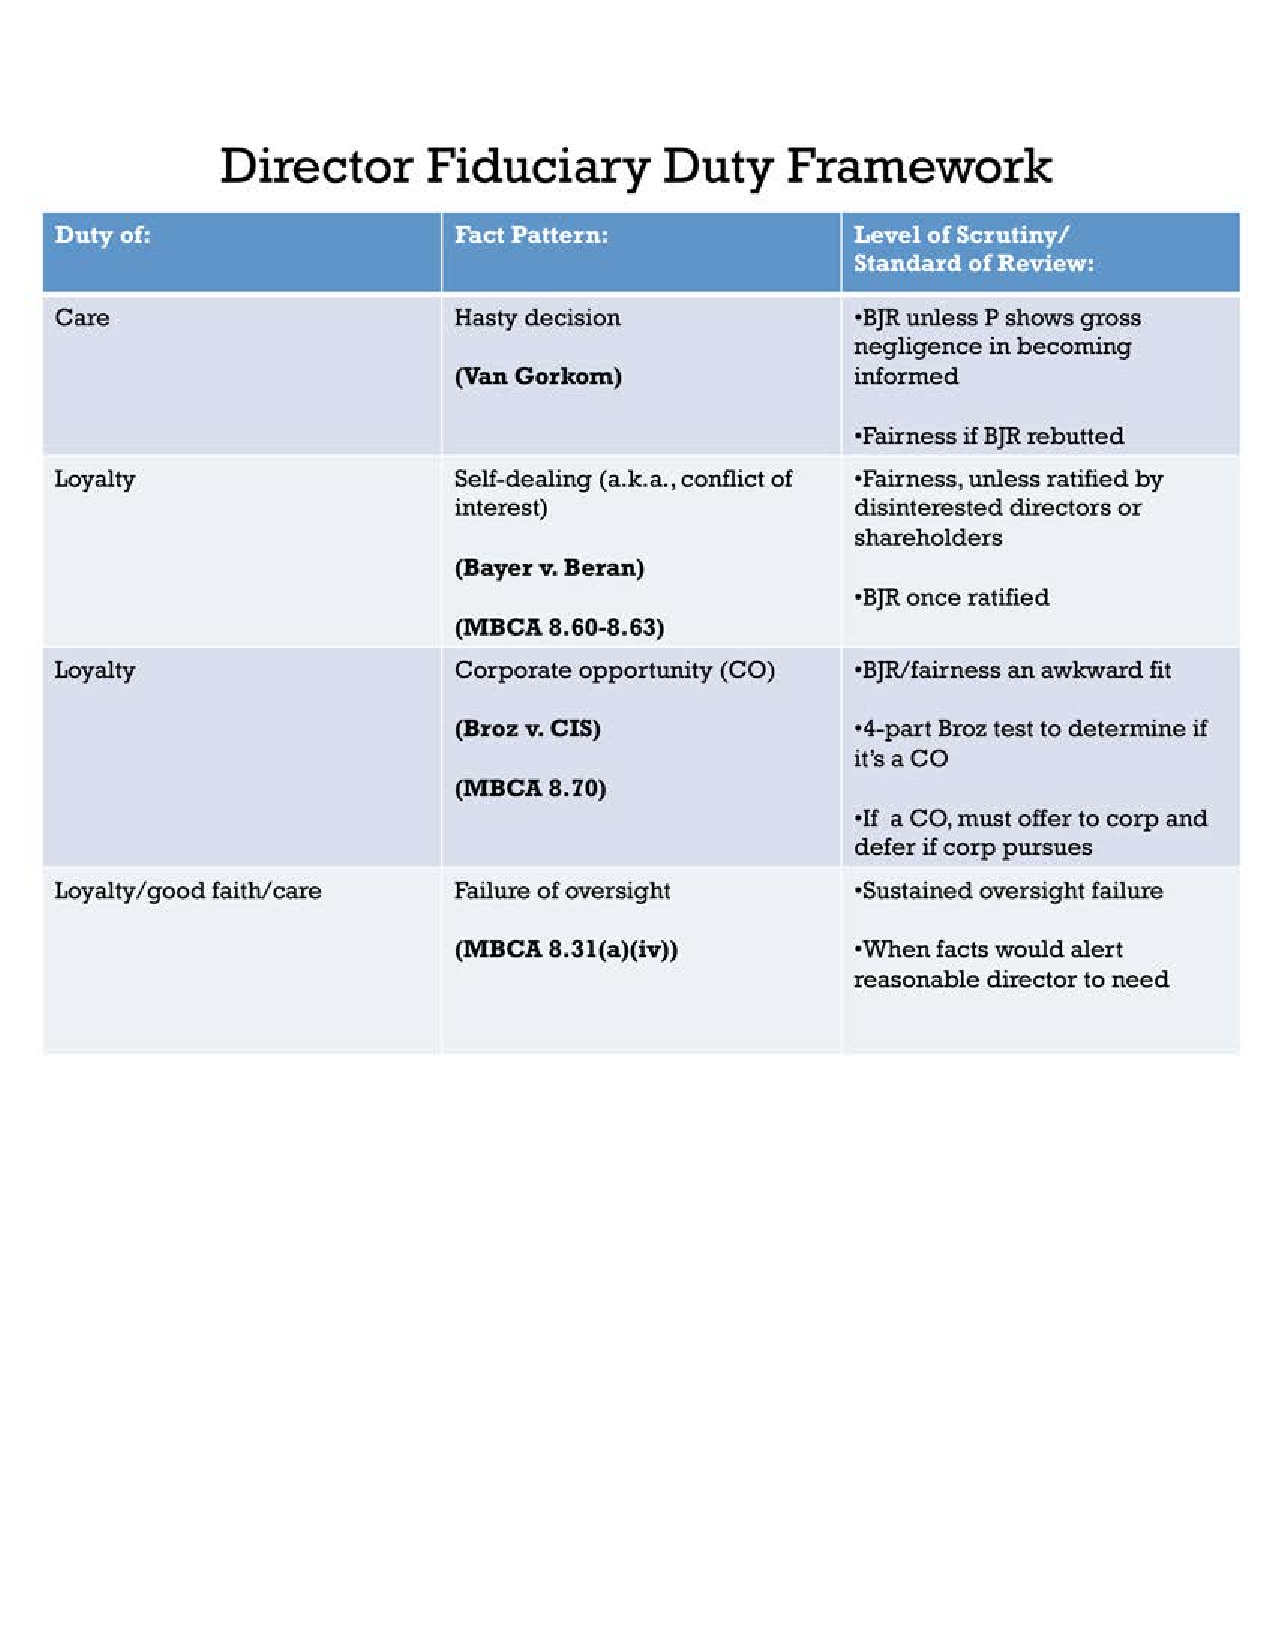
\includepdf{resources/director-fiduciary-duty-framework.pdf}
\end{enumerate}

\newpage

\subsection{Advising Choice of Entity}

\begin{enumerate}
    \item Shareholders vote on: election of directors; removal of directors; 
    mergers, sale of all assets, article amendments, dissolution.
    \item Shareholders \textbf{don't} vote on: election of officers, 
    dividends, ordinary business.
    \item \textbf{Share transferability}: see next page.
\end{enumerate}

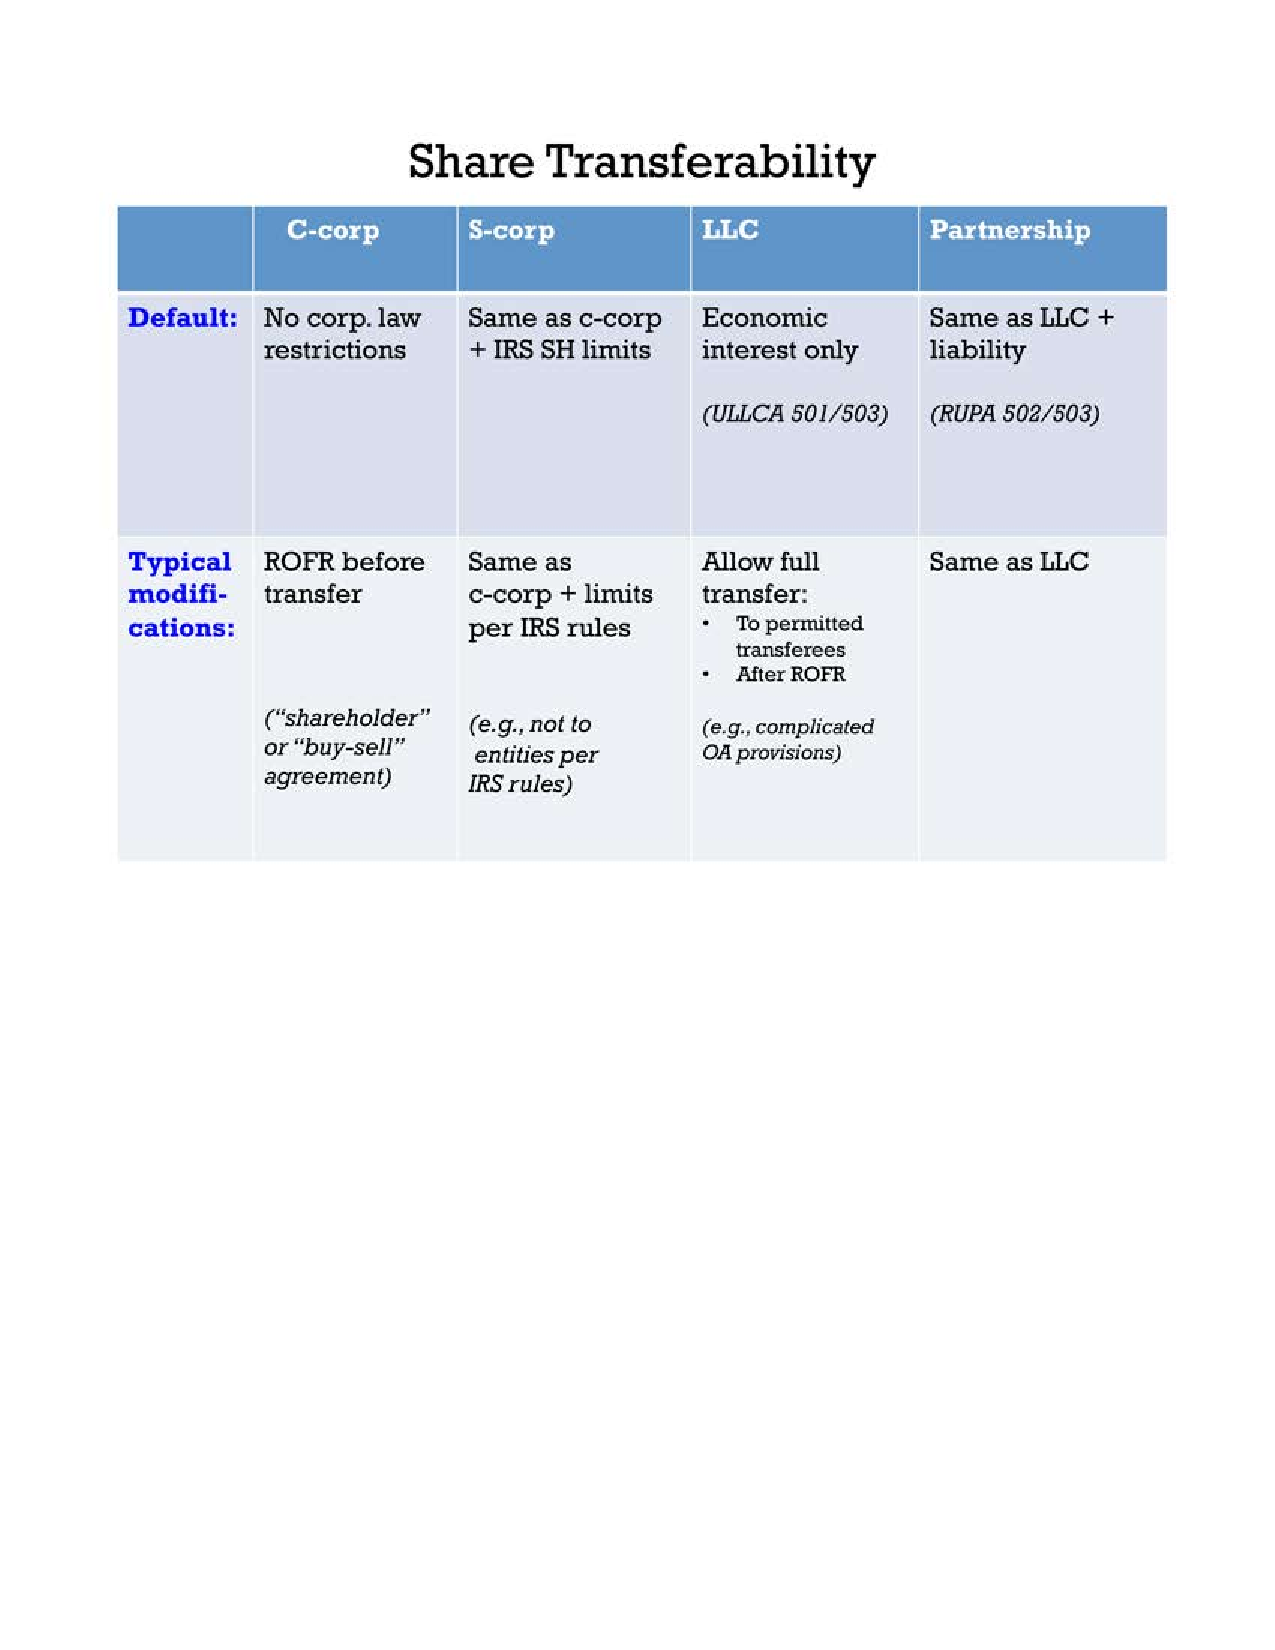
\includepdf{resources/share-transferability.pdf}
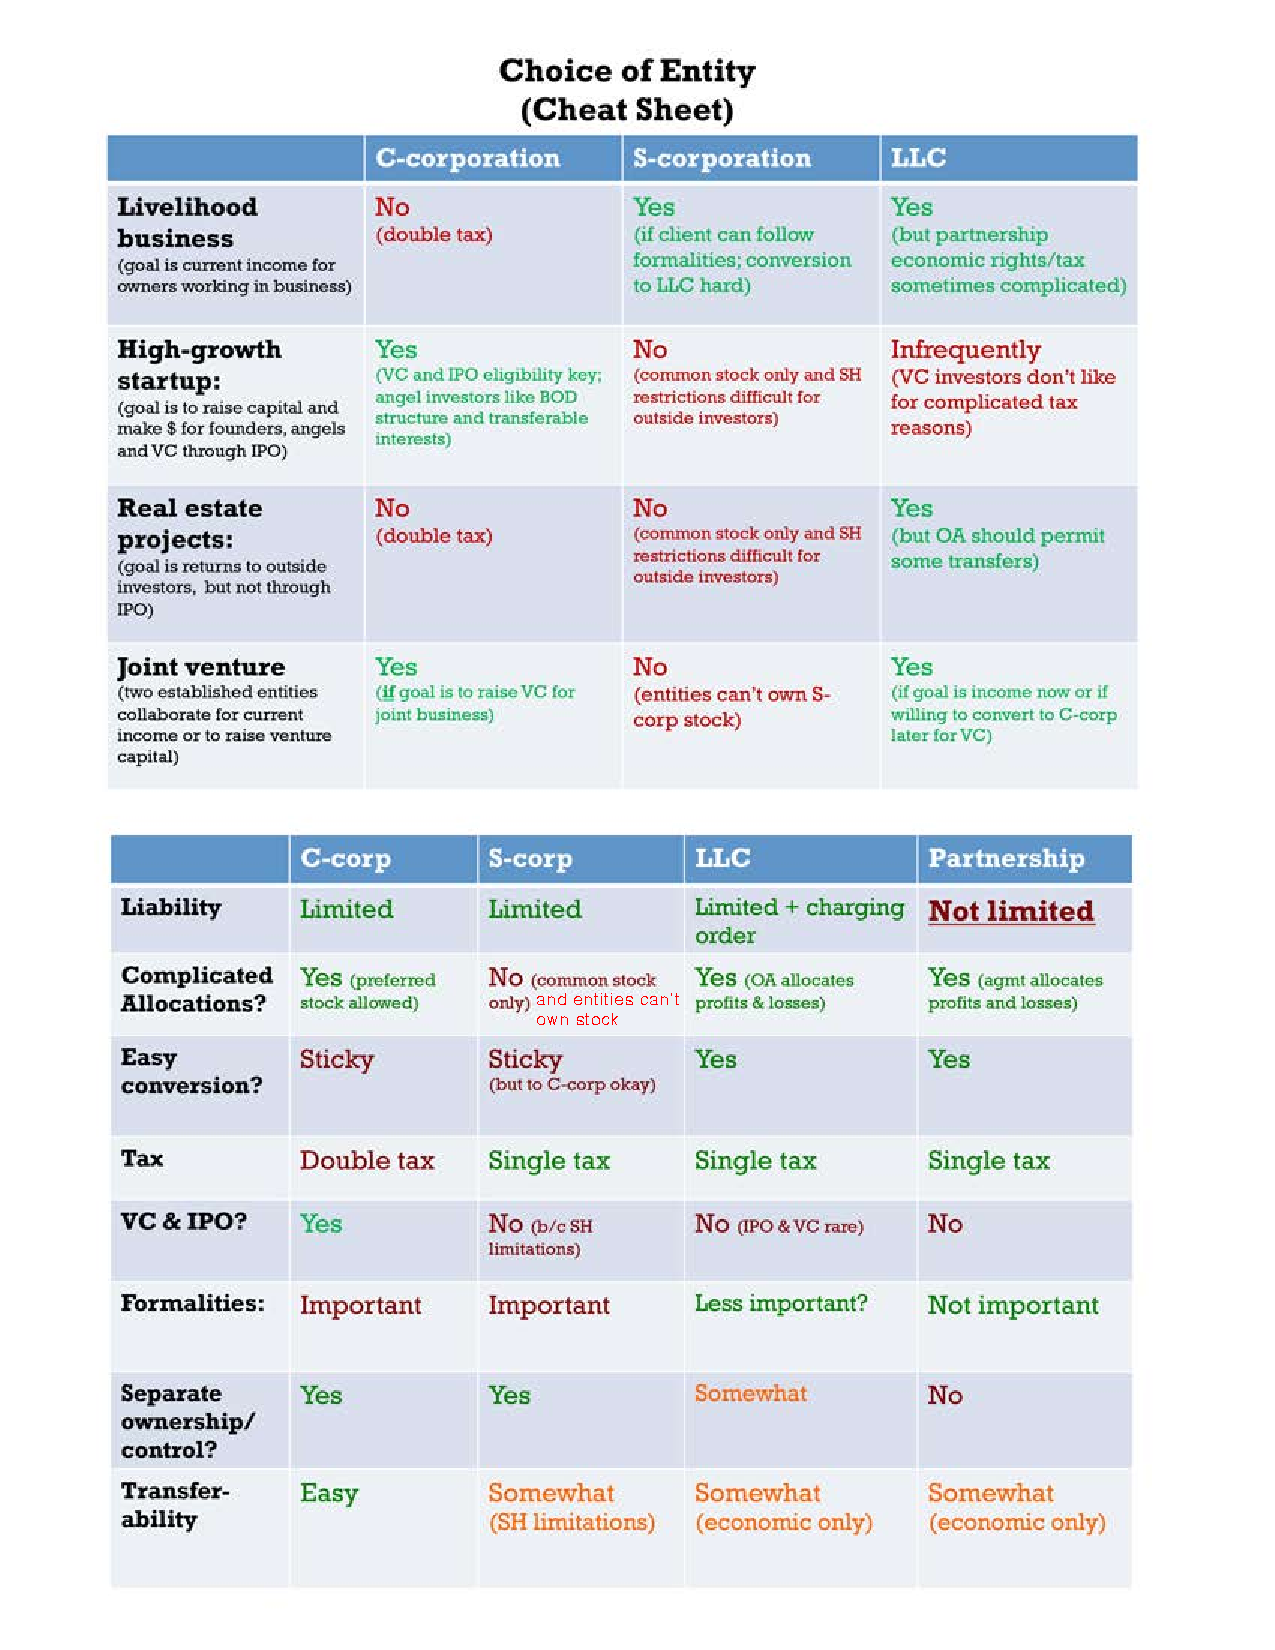
\includepdf{resources/choice-of-entity.pdf}

\newpage

\subsection{Securities}

\begin{enumerate}
    \item A \textbf{security} is a stock, specific instrument (e.g., notes, 
    bonds), or ``investment contract'' (a catch-all). '33 Act \S\ 2(a)(1). 
    Parties' intent is not determinative.
    \item Stock issued by a corporation is \textbf{always a security}. An LLC 
    interest is not categorically a security, but it can be. \emph{Robinson v. 
    Glynn} (the cellphone technology fraud case). % TODO add xref
    \item \textbf{Sources of law}:
    \begin{enumerate}
        \item \textbf{'33 Act}: Securities Act of 1933.
        \item \textbf{'34 Act}: Securities Exchange Act of 1934.
        \item State \textbf{blue-sky laws} (often preempted).
    \end{enumerate}
    \item \textbf{'33 Act}:
    \begin{enumerate}
        \item Regulated securities \textbf{transactions}.
        \item Concerned with the \textbf{primary market}---e.g., an IPO.
        \item \S\ 5 requires \textbf{registration of an offer or sale} of 
        securities, unless an \textbf{exemption} applies. Includes:
        \begin{enumerate}
            \item Sale of stock to \textbf{raise capital}.
            \item Issuance of stock in a \textbf{merger or acquisition}.
        \end{enumerate}
        \item Goals:
        \begin{enumerate}
            \item Mandate \textbf{disclosure} of material information to 
            investors.
            \item Prevent \textbf{fraud}.
        \end{enumerate}
        \item \textbf{Public offering} requires:
        \begin{enumerate}
            \item \textbf{Prospectus}: material information distributed to 
            investors.
            \item \textbf{Registration statement}: prospectus and exhibits 
            to be filed with the SEC.
        \end{enumerate}
        \item \textbf{Exemptions}:
        \begin{enumerate}
            \item \textbf{Private placement exemption}: a transaction not 
            involving a public offering. '33 Act \S\ 4(a)(2). To qualify for 
            the exemption, defendants must show (1) \textbf{actual disclosure} 
            to investors or (2) that investors had \textbf{effective access to 
            all pertinent facts}. \emph{Doran v. Petroleum} (the oil drilling 
            overproduction case). Courts will consider:
            \begin{enumerate}
                \item The number of offerees and their relationships.
                \item The number of units offered.
                \item The size of the offering.
                \item The manner of the offering.
            \end{enumerate}
            \item Exempt \emph{securities} are rare compared to exempt 
            \emph{transactions}.
            \item Exemptions for \textbf{secondary transactions}. Rule 144a.
            \textbf{Remedy} for unregistered and non-exempt transactions: 
            rescission.
        \end{enumerate}
    \end{enumerate}
    \item \textbf{'34 Act}:
    \begin{enumerate}
        \item Governs securities \textbf{markets}.
        \item ``Class'' of securities registered if (1) there are thousands of 
        record shareholders and (2) shares are traded on a public exchange.
        \item Periodic reports, audited finances, internal controls.
        \item Rules for soliciting proxies (see below).
        \item Fraud provisions (see rule 10b-5 below). See also \emph{Robinson 
        v. Glynn} (asserting a 10b-5 violation; the issue was whether 
        the interest was a security).
        \item 
    \end{enumerate}
    \item \textbf{Insider trading}:
    \begin{enumerate}
        \item \textbf{Common law fraud}:
        \begin{enumerate}
            \item Intentional \textbf{false representation}; and
            \item Made to \textbf{induce reliance} by the plaintiff; and
            \item Plaintiff \textbf{actually relied} on the representation; 
            and
            \item Plaintiff \textbf{suffered damages} as a result of the 
            representation.
            \item \textbf{Omissions} are generally not actionable unless (1) 
            what is said becomes \textbf{misleading} or (2) the parties owe 
            \textbf{special duties} to each other as fiduciaries.
        \end{enumerate}
        \item \textbf{Rule 10b-5}:
        \begin{enumerate}
            \item You can't use mail or national securities exchange to do one 
            of the following \textbf{in connection with the purchase or sale 
            of a security}:
            \begin{itemize}
                \item Employ device, scheme, etc. to \textbf{defraud}.
                \item Make \textbf{untrue statement of material fact} or 
                \textbf{omit material fact} necessary to make statements not 
                misleading.
                \item Engage in a fraudulent or deceptive act, practice, etc.
            \end{itemize}
            \item The purpose of the rule is to make sure that all securities 
            investors have ``relatively equal access to 
            information.''\footnote{Casebook p. 470.} All investors should be 
            subject to \textbf{identical market risks}. Those who have 
            \textbf{material inside information} must (1) \textbf{disclose} 
            the information to the public or (2) \textbf{refrain from 
            investing} in the securities concerned. Information is 
            \textbf{material} if it would have a \textbf{substantial effect on 
            the market price of the security}.\footnote{Casebook p. 471.} 
            \emph{SEC v. Texas Gulf Sulphur Co.} (the misleading press release 
            case, holding that the information was material). % TODO xref
            \item Two theories of fraud:
            \begin{itemize}
                \item \textbf{Classical theory}: the \emph{source} of the 
                information acts improperly. The duty to disclose arises from 
                a \textbf{fiduciary relationship}. \textbf{Tippees} receiving 
                confidential information have a duty to disclose only when the 
                insider passed the tip with an \textbf{improper purpose} 
                (i.e., when the insider breached \emph{his} fiduciary duties).  
                \emph{Dirks v. SEC}.
                \item \textbf{Misappropriation}: the \emph{recipient} of 
                information acts improperly. Misappropriation is deception, so 
                it satisfies the requirements of '34 Act \S\ 10(b). It arises 
                when the owner of the information \textbf{trusts} the 
                recipient, and the recipient then \textbf{deceives} the owner 
                to take advantage of the information.  \emph{U.S. v. O'Hagan}. 
                % TODO xref
            \end{itemize}
        \end{enumerate}
    \end{enumerate}
\end{enumerate}

\newpage

\subsection{Public Company Governance}

\begin{enumerate}
    \item \textbf{Proxies}:
    \begin{enumerate}
        \item Shareholders rarely attend meetings because their impact is so 
        small. But meetings can become contentious when insurgents try to 
        \textbf{take control} of the company by electing their own directors, 
        or when an \textbf{issue requiring shareholder approval} is to be 
        decided (e.g., amending the articles or liquidating the firm).
        \item \textbf{Proxy basics}:
        \begin{enumerate}
            \item Incumbent directors solicit shareholders to act as their 
            agent (\textbf{``proxyholder''} or just ``proxy'').
            \item Shareholder appoints the agent with a \textbf{proxy card} 
            (or just ``proxy'').
        \end{enumerate}
        \item \textbf{Proxy fights}:
        \begin{enumerate}
            \item Insurgents solicit their own proxy cards.
            \item Their goal is to gain corporate control or to take some 
            other action to which the incumbents are opposed.
        \end{enumerate}
        \item Incumbents can use company funds to solicit proxies as long as 
        the amounts and methods are reasonable. \emph{Levin v. MGM}.
        \item \textbf{How a proxy fight works}:
        \begin{enumerate}
            \item Company \textbf{issues notice} of annual meeting. One order 
            of business might be to elect directors, which requires a quorum 
            of shareholders to vote in person or by proxy.
            \item Incumbents \textbf{solicit proxies} subject to the '34 Act 
            requirements. Mainly, they must issue a \textbf{proxy statement} 
            containing:
            \begin{enumerate}
                \item Voting information.
                \item Executive compensation information.
                \item Share ownership information.
                \item Cost of proxy solicitation.
            \end{enumerate}
            \item Rule 14a-8 allows \textbf{shareholder proposals} to appear 
            in the company's proxy statement---see below.
            \item How \textbf{insurgents solicit proxies}:
            \begin{enumerate}
                \item Bylaws describe procedures for shareholders to nominate 
                board candidates.
                \item Dissidents \textbf{cannot access the corporation's own 
                proxy statement}, so they run their own campaign at their own 
                expense.
                \item They obtain the shareholder list (see ``shareholder 
                inspection rights'' below), file their proxy solicitation with 
                the SEC, and they engage proxy solicitation firms to deal with 
                large institutional shareholders.
            \end{enumerate}
        \end{enumerate}
    \end{enumerate}
    \item \textbf{Shareholder inspection rights}:
    \begin{enumerate}
        \item Federal proxy rules allow the company to mail the dissidents' 
        proxy materials to shareholders, but \textbf{dissidents want the 
        shareholder lists}, so they resort to \textbf{inspection rights} under 
        state corporation codes. See MBCA \S\S\ 7.20, 16.01--04, 16.20.
        \item Shareholders can inspect shareholder lists for the purpose of 
        making a \textbf{tender offer} because a pending tender offer is a 
        ``business purpose'' and therefore proper. \emph{Crane v. Anaconda}.
        \item The shareholder's purpose for accessing shareholder lists must 
        be relevant to the shareholder's \textbf{``economic interest as a 
        shareholder''}---e.g., his return on investment. Political or ethical 
        purposes are insufficient. \emph{State Ex Rel. Pillsbury v. Honeywell} 
        (the Vietnam munitions case).
        \item \textbf{NOBO lists} must be produced, even if production is 
        burdensome to the company. (``NOBO'' = non-objecting beneficial 
        owners---shareholders who own shares via brokerage houses). 
        \emph{Sadler v. NCR}.
    \end{enumerate}
    \item \textbf{Shareholder proposals}:
    \begin{enumerate}
        \item Rule 14a-8 allows shareholder proposals to appear in the 
        company's proxy statement, subject to several requirements:
        \begin{enumerate}
            \item Only available to owners of more than \$2,000 in stock, 
            held for more than one year.
            \item 500-word supporting statement.
            \item Compliance with SEC policies on misleading statements.
            \item Usually cast as a \textbf{recommendation} because direct 
            shareholder action is improper under state law.
        \end{enumerate}
        \item A company can exclude a shareholder proposal from its proxy 
        statement if it is not \textbf{``significantly related to the issuer's 
        business.''} Rule 14a-8(i)(5). But proposals that are economically 
        insignificant but \textbf{ethically or socially significant} cannot be 
        excluded. \emph{Lovenheim v. Iroquois} (the foie gras case).
        \item A company can exclude shareholder proposals if they ``relate[] 
        to an election for membership'' on the board (Rule 14a-8(i)(8)), but 
        not if they relate to \textbf{election procedure}. \emph{AFSCME v. 
        AIG}.
        \item Shareholder proposals can aim to make \textbf{process-oriented 
        modifications to the bylaws}, but some bylaw modifications are not 
        allowed because they would unduly restrict the board. \emph{CA v. 
        AFSCME}.
    \end{enumerate}
\end{enumerate}

\newpage

\subsection{Mergers and Acquisitions}

\begin{enumerate}
    \item \textbf{Two-tiered front-loaded cash tender offer}:
    \begin{enumerate}
        \item You own a few shares in a company. Each share is worth \$50.
        \item T. Boone Pickens offers to buy the first 51\% of the company's 
        shares at \$65/share. Then, he'll merge the company with his own firm, 
        offering \$55 in junk bonds to the company's remaining shareholders.
        \item You don't own enough shares to block the deal. So, if you're 
        rational, you'll sell your shares for \$65.
        \item Thus, the offer coerces shareholders into selling.
    \end{enumerate}
    \item The \textbf{\emph{Unocal} test}:
    \begin{enumerate}
        \item \textbf{Triggers}: board takes \textbf{defensive measures} in 
        response to a hostile deal.
        \item \textbf{Test}:
        \begin{enumerate}
            \item \textbf{Motive}: did the board identify a danger to 
            corporate policy or effectiveness, through good faith and 
            reasonable investigation, preferably by outside directors? Proper 
            motives can include:
            \begin{enumerate}
                \item Inadequacy of the amount or form of consideration.
                \item Timing of the offer.
                \item Risk that the offer will prevent other deals from 
                getting done.
                \item Non-shareholder effects.
                \item Impact on long-term strategic vision (e.g., journalistic 
                integrity).
            \end{enumerate}
            \item \textbf{Proportionality}: is the defensive measure 
            reasonable in proportion to the threat posed? Reasonable measures 
            can include:
            \begin{enumerate}
                \item Avoiding subsidizing the threatening offer (e.g., 
                \emph{Unocal}).
                \item (Need not be narrowly tailored.)
            \end{enumerate}
        \end{enumerate}
    \end{enumerate}
    \item The \textbf{\emph{Revlon} test}:
    \begin{enumerate}
        \item \textbf{Triggers}: board takes action that makes the 
        \textbf{breakup of the company inevitable}, such as:
        \begin{enumerate}
            \item Self-initiated \textbf{sale} of the company for 
            \textbf{cash} (but not for stock); or
            \item Stock-for-stock \textbf{deal} resulting in a 
            \textbf{controlling shareholder} (including shareholders under the 
            control of another, but not if there is not a controlling 
            shareholder).
            \item White knight deals (e.g., \emph{Revlon}).
        \end{enumerate}
        \item \textbf{Not triggers}:
        \begin{enumerate}
            \item \textbf{Simple refusal} of unsolicited offer.
            \item Deal where control remains in \textbf{unaffiliated hands} 
            (i.e., the market at large).
        \end{enumerate}
        \item \textbf{Test}:
        \begin{enumerate}
            \item The board must take steps to \textbf{maximize the short-term 
            value} of the deal.
        \end{enumerate}
    \end{enumerate}
\end{enumerate}

\subsection{Corporate Litigation}

\begin{enumerate}
    \item See chart on following page.
    \item \textbf{Direct vs. derivative claims}:
    \begin{enumerate}
        \item \textbf{Direct}: shareholders allege that the corporation has 
        \textbf{injured them directly}. The corporation pays damages to the 
        shareholder.
        \item \textbf{Derivative}: shareholders \textbf{vindicate a duty owed 
        to the corporation}---e.g., officer/director fiduciary duties, or the 
        obligations of a third party to the corporation. Shareholders bring 
        the suit on behalf of the corporation.
    \end{enumerate}
    \item \textbf{Demand}: before bringing a derivative suit, shareholders 
    must \textbf{demand} that the corporation bring the suit itself. The 
    shareholder can only bring a derivative suit once the corporation 
    \textbf{refueses} the demand.
    \item In some scenarios, demand is \textbf{excused} if it would be 
    \textbf{futile}.
    \item Delaware demand requirement (\emph{Grimes}):
    \begin{enumerate}
        \item Before bringing a derivative suit, the shareholder must:
        \begin{enumerate}
            \item \textbf{Make a demand}; or
            \item Argue that demand is \textbf{excused as futile} because:
            \begin{enumerate}
                \item Majority of the board has a \textbf{material financial 
                or familial interest}; or
                \item The board is \textbf{not independent} for another 
                reason, such as domination or control by a non-independent 
                director; or
                \item The underlying transaction is not fair under the 
                business judgment rule.
                \item (Once a shareholder makes a demand, he can no longer 
                argue that demand is excused. \emph{Grimes}.)
                \item (New York also excuses demand when the directors did not 
                fully inform themselves. \emph{Marx}.)
            \end{enumerate}
        \end{enumerate}
        \item If the board \textbf{refuses the demand}, the board's decision 
        is entitled to the business judgment rule, but the shareholder can 
        argue that the board's refusal was \textbf{wrongful} because the board 
        did not act independently or with due care.
    \end{enumerate}
    \item Corporations can appoint \textbf{special litigation committees 
    (SLCs)} to determine whether derivative litigation should proceed.
    \item Delaware two-step standard for reviewing SLC recommendations 
    (\emph{Zapata}):
    \begin{enumerate}
        \item First, did the SLC act \textbf{independently} and \textbf{in 
        good faith}? On what bases did the committee make its recommendation? 
        (The corporation has the burden of proving independence, good faith, 
        and reasonable investigation.)
        \item Second, the court can apply \textbf{its own business judgment} 
        as to whether the case should be dismissed. (The purpose of this step 
        is to allow meritorious suits to go forward and to account for the 
        structural bias problem.)
    \end{enumerate}
    % FIXME add indemnification/waltuch
\end{enumerate}

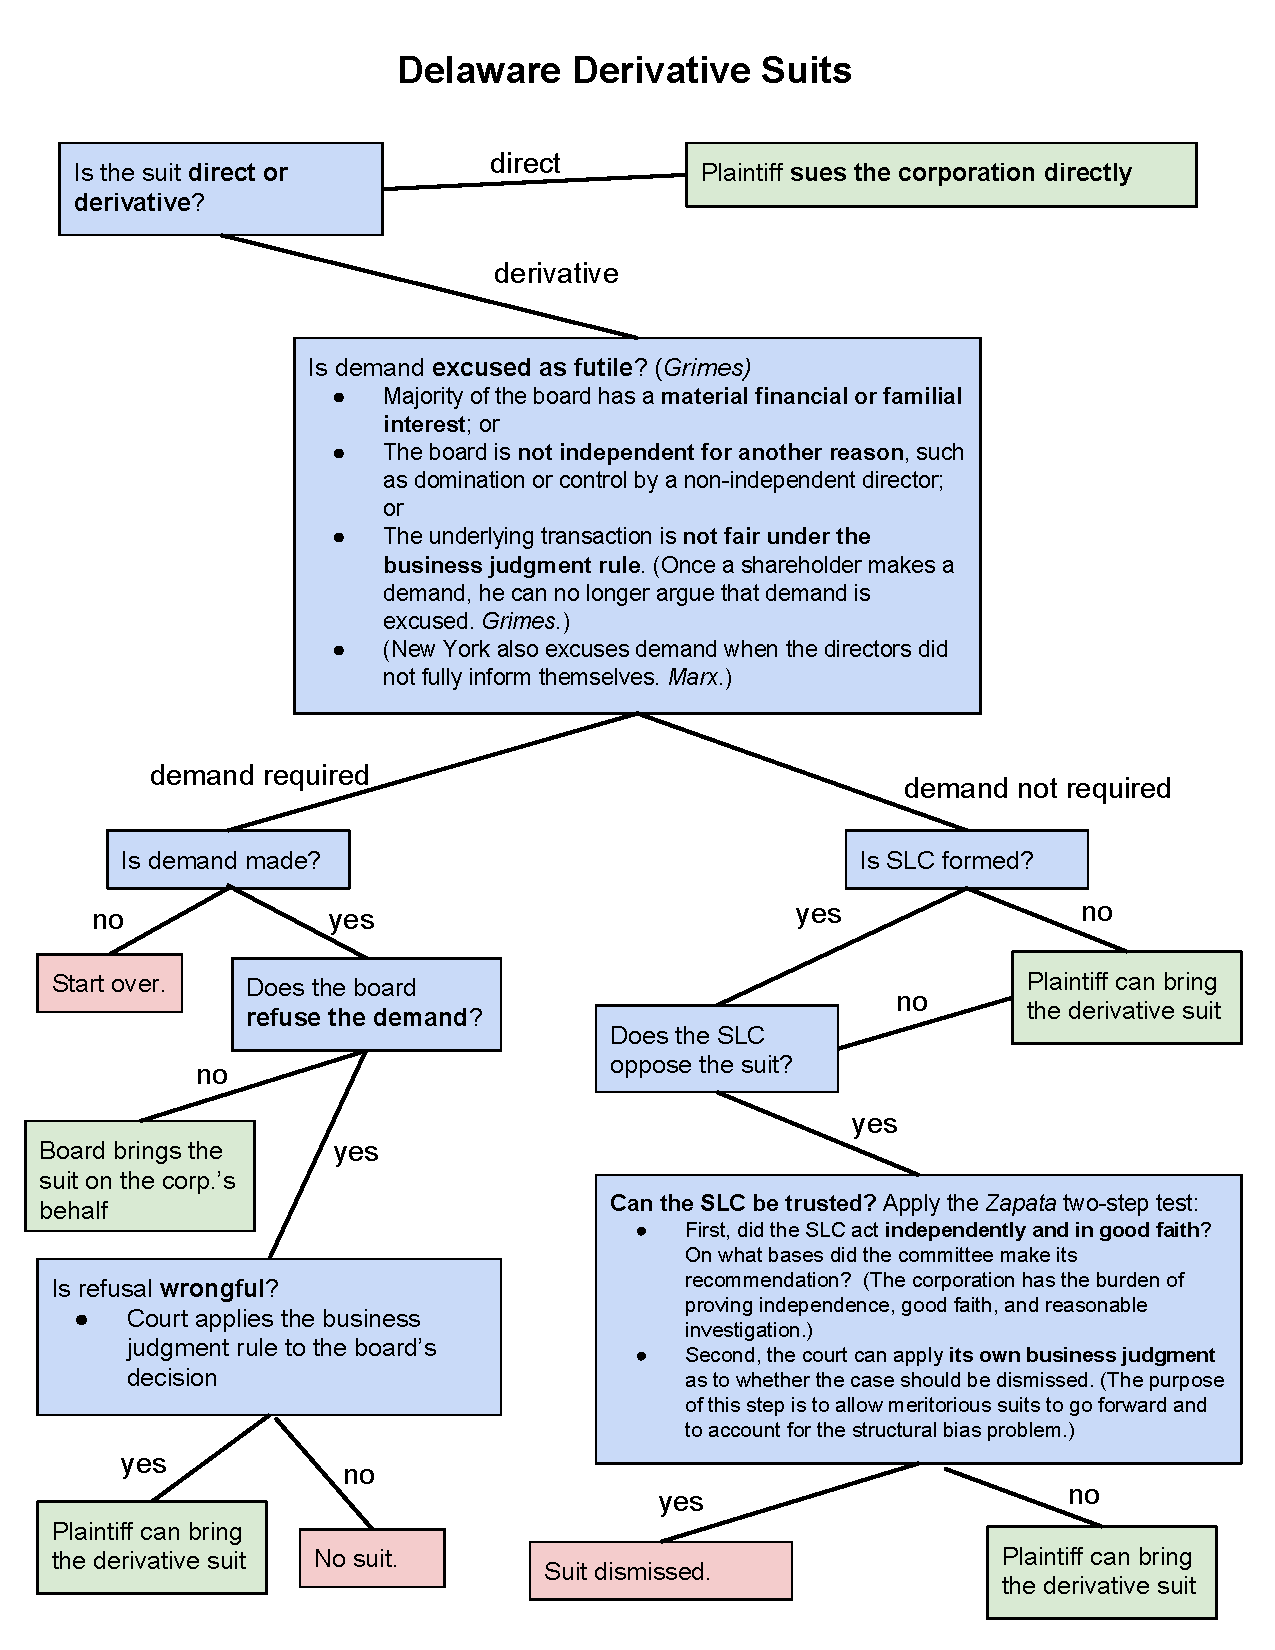
\includepdf{resources/delaware-derivative-suits.pdf}
